\documentclass[oneside,a4paper,14pt,final]{extreport}

\usepackage{essay}
\usepackage{bigints}
\usepackage{setspace}
%%%%%%%%%%%%%%%%%%%%%%%%%%%%%%%%%%%%%%%%%%%%%%%%%%%
%                                                 %
%              declare math operators             %
%                                                 %
%%%%%%%%%%%%%%%%%%%%%%%%%%%%%%%%%%%%%%%%%%%%%%%%%%%
% https://tex.stackexchange.com/questions/67506/newcommand-vs-declaremathoperator
% \DeclareMathOperator{\End}{End}
\DeclareMathOperator*{\argmax}{arg\,max}
\DeclareMathOperator*{\argmin}{arg\,min}
\DeclareMathOperator*{\sign}{sign}
\newcommand{\introname}{ВВЕДЕНИЕ}
\usepackage[font=small]{caption}
\graphicspath{ {./images/} }
\addbibresource{./library.bib}
\begin{document}
\begin{titlepage}
\newpage

{\setstretch{1.0}
\begin{center}
    Федеральное государственное автономное образовательное учреждение высшего образования «Национальный исследовательский университет «Высшая школа экономики»
\\
\bigskip
Факультет компьютерных наук \\
Прикладная математика и информатика \\
\end{center}
}

\vspace{8em}

\begin{center}
{\Large ДИПЛОМНАЯ РАБОТА}\\
\textsc{\textbf{
Исследовательский проект на тему
\linebreak
"Замена лица (FaceSwap) с помощью генеративных моделей"}}

\end{center}

\vspace{2em}

{\setstretch{1.0}
\hfill\parbox{16cm}{
\hspace*{5cm}\hspace*{-5cm}Выполнил студент группы мИИАД22, 2 курс,\\
 Рябыкин Алексей Сергеевич\\
 
\hspace*{5cm}\hspace*{-5cm}Научный руководитель:\\
научный сотрудник Аланов Айбек \\

%\hspace*{5cm}\hspace*{-5cm}Куратор:\hfill < степень>, <звание>, <ФИО полностью>\\

}
}

\vspace{\fill}

\begin{center}
Москва 2024
\end{center}

\end{titlepage}
%%%%%%%%%%%%%%%%%%%%%%%%%%%%%%%%%%%%%%%%%%%%%%%%%%% 
\chapter*{РЕФЕРАТ}

\bigskip\par
Дипломная работа содержит \pageref*{LastPage}~страниц, N~рисунок, N~таблицу, N использованных источников.

\bigskip\par
Face swap, Deepfakes, ДИФФУЗИОННЫЕ МОДЕЛИ, ГЕНЕРАТИВНЫЕ МОДЕЛИ

\bigskip\par
Дипломная работа посвящена исследованию современных методов замены лиц на изображения с помощью диффузионных моделей. Исследована проблема

\bigskip
Теоретическая часть работы содержит исследовательский обзор статей о диффузионных моделях для задачи замены лиц на изображении (Face swap)...

\bigskip
В практической части содержатся результаты поставленных экспериментов, их анализ и постановка последующих исследований.
\thispagestyle{empty} % unnumbered page

{\linespread{0.9}\tableofcontents}

\chapter{\introname}
\par
TBD
%%%%%%%%%%%%%%%%%%%%%%%%%%%%%%%%%%%%%%%%%%%%%%%%%%%
{\CenterChapterHeading\chapter*{ОСНОВНАЯ ЧАСТЬ}
\addcontentsline{toc}{chapter}{ОСНОВНАЯ ЧАСТЬ}
\newpage
}
%%%%%%%%%%%%%%%%%%%%%%%%%%%%%%%%%%%%%%%%%%%%%%%%%%%
\section{ТЕОРЕТИЧЕСКАЯ ЧАСТЬ}
\vspace{-1.3cm}

% \input{./theory/task.tex}
% \input{./theory/preprocessing.tex}
% \input{./theory/methods.tex}
% \input{./theory/external_data.tex}
\subsection{Обзор литературы}

\subsubsection{Общие сведения о диффузионных моделях}
\par
Долго лидирующие на поприще генерации изображений генеративно-состязательные сети обладают набором проблем, с которыми боролось и продолжает бороться научное сообщество. Основными проблемами, сохранившимися до сих пор, являются нестабильность обучения \cite{kodali2017convergence}, решаемая с помощью спектральной нормализации \cite{miyato2018spectral}, контролирующей константу Липшица, вводя ограничение весов, для стабилизации обучения дискриминатора; Mode Collapse \cite{thanhtung2020catastrophic}. Последняя является одной из главных проблем моделей такого типа. Проблема заключается в том, что в процессе обучения генератор приходит к состоянию, при котором генерируется лишь ограченный (существенно меньший оригинального пространства изображений) набор выходов. Предлагаемые решения этой проблемы -- WGAN \cite{arjovsky2017wasserstein} (авторы используют метрику Вассерштейна внутри лосс-функции, тем самым мотивируя дискриминатор выявлять повторяющие выходы, в которых стабилизировался генератор) и UGAN \cite{metz2017unrolled} (также адаптация функции потерь, однако теперь с оценкой выходов генератора на основе предсказаний будущих версий дискриминатора).

\par
В отличие от генеративно-состязательных сетей эти же проблемы не свойственны новому классу моделей -- диффузионным моделям. В оригинальной статье \cite{sohldickstein2015deep} авторы утилизируют идею из статистической термодинамики. Главной целью авторы видят определение двух процессов: итеративный диффузный процесс, который преобразует любое комплекное распределение данных в более простое и контролируемое, постепенно уменьшая SNR (signal-to-noise ratio), а также параметризованный обратный диффузионный процесс, обучаемый итеративно моделировать целевое распределение.


\textbf{Прямой процесс}

\par
Рассмотрим набор данных из сложно контролируемого целевого распределения: $X = (x^1, \ldots, x^n)$. Построим прямой процесс диффузии, постепенно зашумляющий данные из целевого распределения (уменьшая SNR).
\[
    \begin{array}{c}
        x^i_0 \to x^i_1 \to \ldots \to x^i_T\\
        x^i_{t} = \sqrt{1-\beta_t}\cdot x^i_{t-1} + \sqrt{\beta_t}\cdot \epsilon, \hspace*{0.5cm} \epsilon \sim \mathcal{N}(\epsilon| \ 0, \ I)
    \end{array}
\]
где $\beta_t$ -- скорость диффузии на шаге $t$, $x^i$ -- семпл из выборки (сейчас и далее просто $x$). Этот прямой диффузионный процесс может быть записан в следующем виде:
\begin{equation}
    q(x_{t}|x_{t-1}) = \mathcal{N}(x_{t} \vert \sqrt{1 - \beta_t}x_{t-1}, \beta_t I)
    \label{eq:forward_process}
\end{equation}
\begin{figure}[H]
    \centering
    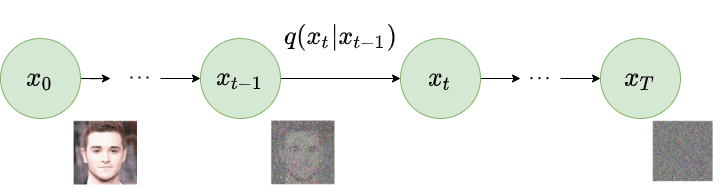
\includegraphics[scale=0.5]{forward-diffusion.png}
    \caption{Прямой процесс диффузии \cite{ho2020denoising}}
    \label{fig:forward_process}
\end{figure}
Используя трюк с репараметризаций можно получить явное выражение для семплирования на каждом шаге диффузии (\hyperref[AppendixA]{ПРИЛОЖЕНИЕ 1}):
\begin{equation}
    x_t \sim q(x_t| x_0) = \mathcal{N}(x_t\vert \sqrt{\overline{\alpha}_t} x_0, \ (1 - \overline{\alpha}_t)I),    
    \label{eq:any_step}
\end{equation}
где $\overline{\alpha_t} = \prod_{s=0}^{t} (1 - \beta_t)$. Из последнего выражения нетрудно заметить, что при $T \to \infty \Longrightarrow \overline{\alpha}_T \to 0$  генерируемый семпл будет иметь стандартное нормальное распределение $x_T \sim \mathcal{N}(x^T\vert 0, I)$. 

\textbf{Обратный процесс}

Построив обратный процесс: $q(x_{t-1}\vert x_t)$ будет возможно воссоздать истинную выборку по входному сигналу гауссова шума. В условиях выбора малых $\beta_t$ можно гарантировать, что $q(x_{t-1}| x_t)$ также гауссово распределение. Однако, оценка $q(x_{t-1}\vert x_t)$ невозможна без генеральной совокупности. В статье \cite{sohldickstein2015deep} предлагается параметризовать оценку условной вероятности $p_\theta$ для запуска процесса обратной диффузии: 
\begin{equation}
    p_\theta(x_{t-1}\vert x_t) = \mathcal{N}(x_{t-1}\vert \mu_\theta(x_t, t), \Sigma_\theta(x_t, t))    
\end{equation}
\begin{figure}[H]
    \centering
    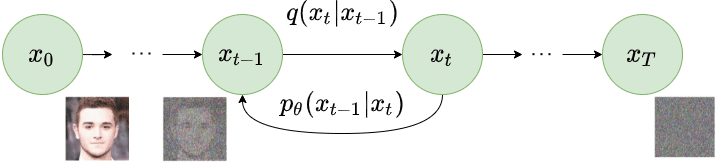
\includegraphics[scale=0.5]{reverse-diffusion.png}
    \caption{Обратный процесс диффузии \cite{ho2020denoising}}
    \label{fig:reverse_process}
\end{figure}

% не до конца понял
Обратная условная вероятность $q(x_{t-1}\vert x_t)$ контролируема, если обусловлена на $x_0$:
\begin{equation}
    q(x_{t-1}\vert x_t, x_0) = \mathcal{N}(x_{t-1}, \tilde{\mu}(x_t, x_0), \tilde{\beta}_t  I)  
    \label{eq:controlable_condition}
\end{equation}
причем из \ref{eq:any_step} следует можно выразить:
\[
    \begin{array}{c}
        \tilde{\beta}_t = \dfrac{1 - \overline{\alpha}_{t-1}}{1 - \overline{\alpha}_t} \cdot \beta_t,  \\[0.5cm]
        \tilde{\mu}_t(x_t, x_0) = \dfrac{}{} x_0 + \dfrac{\sqrt{\alpha_t}(1 - \overline{\alpha}_{t-1})}{1-\overline{\alpha}_t} x_t
    \end{array}
\]
Пользуясь результатами \hyperref[AppendixA]{ПРИЛОЖЕНИЕ 1.} можно выразить:
\[
    x_0 = \dfrac{1}{\sqrt{\overline{\alpha}_t}} (x_t - \sqrt{1 - \overline{\alpha}_t \epsilon})  
\]
Собирая вместе два последних выражения, можем получить среднее для произвольного шага, зависящее от $x_t$:
\[
    \tilde{\mu}_t(x_t) = \dfrac{1}{\sqrt{\alpha_t}} \left(x_t - \dfrac{\beta_t}{\sqrt{1 - \overline{\alpha}_t}}\epsilon\right)
\]
В статье \cite{ho2020denoising} предлагается использовать нейронную сеть для оценки шума:
\[
    \tilde{\mu}_\theta(x_t, t) = \dfrac{1}{\sqrt{\alpha_t}}\left(x_t - \dfrac{\beta_t}{\sqrt{1 - \overline{\alpha}_t}}\epsilon_\theta(x_t, t)\right)  
\]
Тогда функция ошибки (подробнее в \hyperref[AppendixC]{ПРИЛОЖЕНИЕ 3.}) может быть выражена:
\[
    L_t = \mathbb{E}_{x_0, t, \epsilon}\left[\dfrac{1}{2||\Sigma_\theta(x_t, t)||_2^2} ||\tilde{\mu}_t - \tilde{\mu}_\theta(x_t, t)||_2^2\right] = \mathbb{}_{} \left[\dfrac{1}{2||\Sigma_\theta(x_t, t)||_2^2} ||\epsilon_t - \epsilon_\theta(\sqrt{\overline{\alpha}_t}x_0 + \sqrt{1 - \overline{\alpha}_t}\epsilon, t)||^2\right]
\]
В статье \cite{ho2020denoising} авторы обнаружили, что обучение модели лучше работает с упрощенным лоссом, с опущенным весовым членом
\[
    L_t^* = \mathbb{E}_{x_0, t, \epsilon}\left[||\epsilon_t - \epsilon_\theta(\sqrt{\overline{\alpha}_t}x_0 + \sqrt{1 - \overline{\alpha}_t}\epsilon, t)||^2\right]  
\]
Но в \cite{nichol2021improved} авторы показывают, что если учить оценку ковариационной матрицы, то результат будет лучше.
\begin{figure}[H]
    \centering
    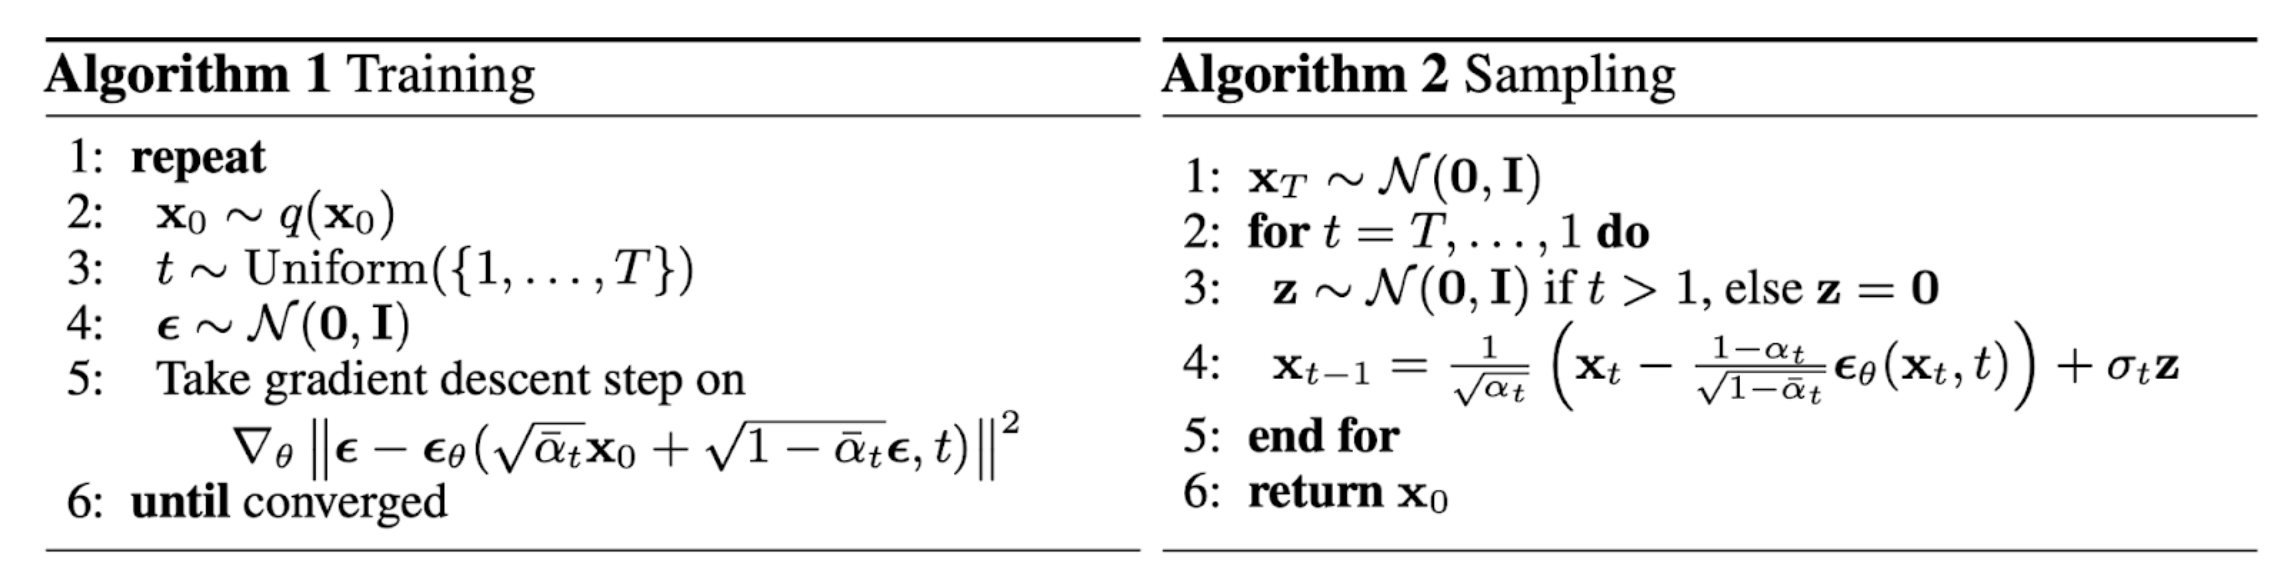
\includegraphics[scale=0.4]{DDPM-algo.png}
    \caption{Алгоритмы обучения и семплирования \cite{ho2020denoising}}
    \label{fig:algo_ddpm}
\end{figure}

% TODO: sheduling \beta_t
% TODO: архитектура


% не до конца понял
% \par
% Динамика Ланжевена \cite{10.5555/3104482.3104568} позволяет сэмплировать из плотности распределения используя только градиенты $\dfrac{\partial}{\partial x} \log p(x)$



% Процедура \ref{eq:Langevene} представляет собой градиентный подъем, который направлен на нахождение моды распределения, однако, что является большим преимуществом перед генеративно-состязательными сетями: происходит зашумление градиента, что релаксирует высокие значения плотности распределения. 

\par

% ! дописать


\subsubsection{Обуславливаемые диффузионные модели (Conditioned diffusion models)}
\par

В статье \cite{rombach2022highresolution} предлагается модель латентной диффузии. Авторы представляют процесс диффузии не в пространстве пикселей, а в пространстве латентных эмбеддингов, полученных с помощью автоэнкодера (VQ-VAE). Авторы обнаружили, что даже агрессивная компрессия сохраняет семантическую и концептуальную информацию \ref{fig:image-distortion-rate}. Поэтому они сначала убирают избыточность (компрессируют) с помощью автоэнкодера, а затем манипулируют/генерируют семантические понятия с помощью процесса диффузии на выученном латентном уровне. Энкодер $\mathcal{E}$ используется для компрессии входных изображений в латентные эмбеддинги: $z = \mathcal{E}(x^{H\times W\times 3}) \in \mathbb{R}^{h\times w\times c}$
\begin{figure}[H]
    \centering
    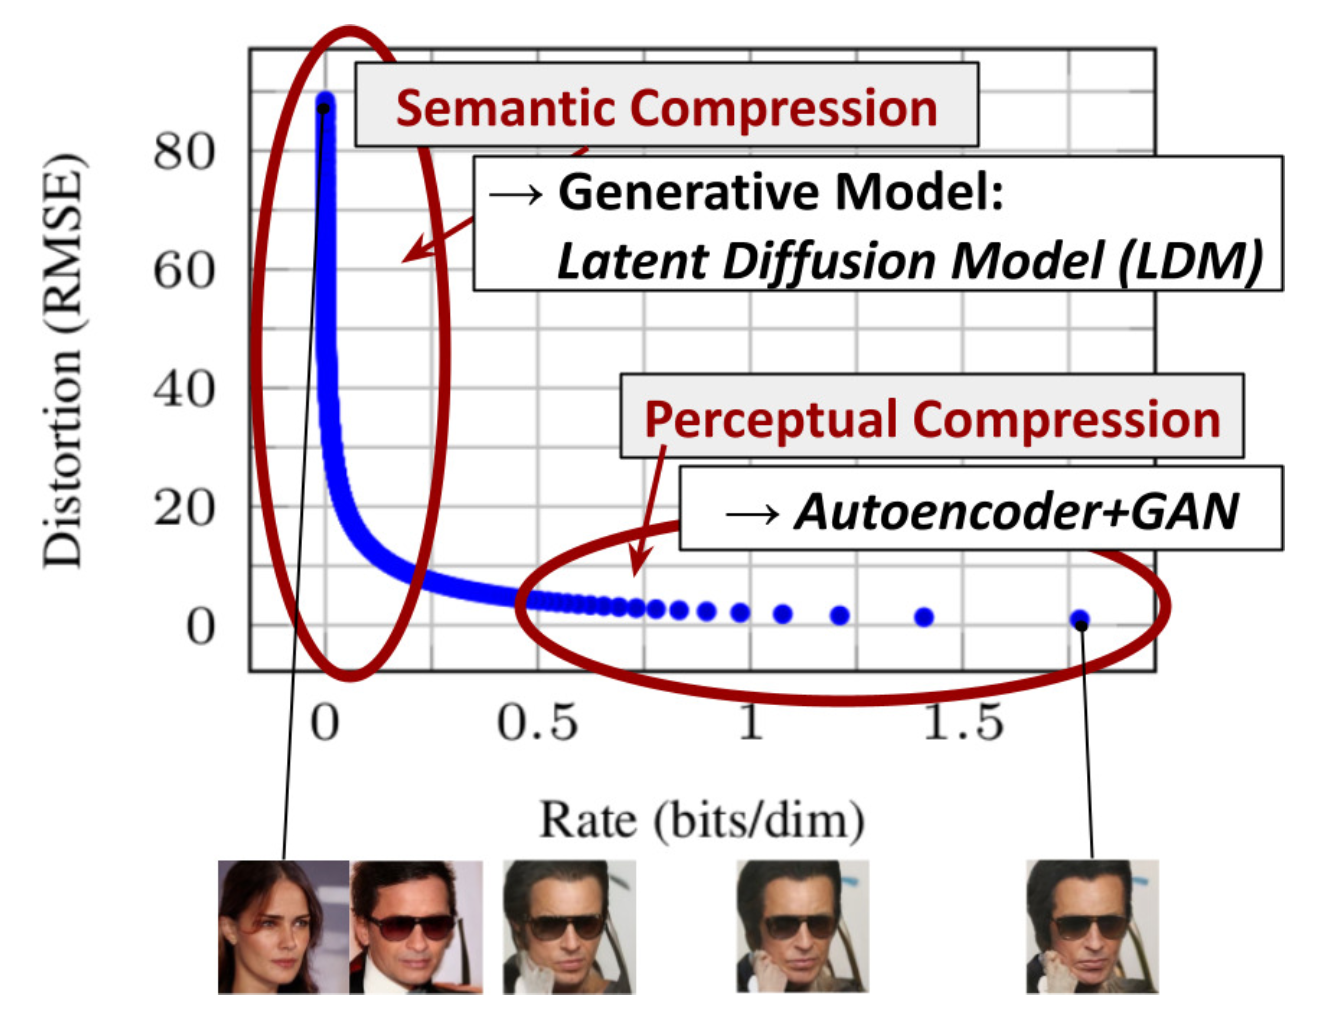
\includegraphics[scale=0.4]{image-distortion-rate.png}
    \caption{Trade-off между сжатием и искажениями \cite{rombach2022highresolution}}
    \label{fig:image-distortion-rate}
\end{figure} 

% ! дописать
В \cite{ruiz2023dreambooth} предлагается использование концептов. 




\subsubsection{Обучение моделей}
\par

\subsubsection{Задача замены лиц (Face swap)}

\par

\subsection{Особенности поставленных экспериментов}
\subsubsection{}
\par

\section{ПРАКТИЧЕСКАЯ ЧАСТЬ}
\vspace{-1.3cm}

\subsection{Используемые инструменты}

\begin{multicols}{3}
\begin{itemize}
 \item Python 3


 \item PyTorch


 \item TorchVision


 \item Matplotlib


 \item hugging-face


 \item Plotly


 \item transformers


 \item TorchIntegral


\item TorchPruning

\item diffusers

\item wandb
\end{itemize}
\end{multicols}


\subsection{Экспериментальные результаты}
\par

\subsection{Выводы}
\par

\subsection{Дальнейшая работа}
\par


\addtocategory{SourcesGOST}{gagar}
\chapter{СПИСОК ИСПОЛЬЗОВАННЫХ ИСТОЧНИКОВ}
% \vspace{-1.0cm}
\begingroup
\let\clearpage\relax
\printbibliography[category=SourcesGOST, title=""]
\vspace{-1.5cm}
\printbibliography[notcategory=SourcesGOST, title=""]
\endgroup
%%%%%%%%%%%%%%%%%%%%%%%%%%%%%%%%%%%%%%%%%%%%%%%%%%%
{\CenterChapterHeading\chapter*{ПРИЛОЖЕНИЯ}
\addcontentsline{toc}{chapter}{ПРИЛОЖЕНИЯ}
\newpage
}
\phantomsection
{\NonNumberedSection\section*{ПРИЛОЖЕНИЕ 1}}
\addcontentsline{toc}{section}{ПРИЛОЖЕНИЕ 1}
\pagestyle{supplement1}
\label{AppendixA}

\textbf{Явное выражение для семплирования на произвольном шаге диффузии}

% TODO: Расписать подробнее, если останется время [DONE]
Рассмотрим выражение \ref{eq:forward_process}. Положим $\alpha_t = 1 - \beta_t$ и $\overline{\alpha}_t = \prod_{s=0}^{t} \alpha_s$. Рекурсивно применяя трюк с репараметризацией:
\[
    \begin{array}{c}
        x_t = \sqrt{1 - \beta_t}x_{t-1} + \sqrt{\beta_t}\epsilon_{t-1} = \sqrt{\alpha_t\alpha_{t-1}}x_{t-2} + \sqrt{1 - \alpha_t\alpha_{t-1}}\epsilon_{t-2} = \ldots \\
        \ldots = \sqrt{\overline{\alpha}_t} x_0 + \sqrt{1 - \overline{\alpha}_t} \epsilon_0,
    \end{array}
\]
где $\epsilon_{t-1}, \varepsilon_{t-2}, \ldots \sim \mathcal{N}(0, I)$, $\overline{\epsilon}_{t-2}$ смесь нормальных распределений 
\[
    \overline{\epsilon}_{t-2} \sim \mathcal{N}(0, \sqrt{(1-\alpha_t) + \alpha_t(1-\alpha_{t-1})}I) = \mathcal{N}(0, \sqrt{1 - \alpha_t\alpha_{t-1}})
\]
Обычно по мере зашумления используется больший шаг зашумлений, т.е.:
\[
    \begin{array}{c}
        \beta_1 < \beta_2 < \ldots < \beta_T,\\
        \overline{\alpha_1} > \overline{\alpha_2} > \ldots > \overline{\alpha_T}.
    \end{array}  
\]

\newpage
\phantomsection
{\NonNumberedSection\section*{ПРИЛОЖЕНИЕ 2}}
\addcontentsline{toc}{section}{ПРИЛОЖЕНИЕ 2}
\pagestyle{supplement2}
\label{AppendixB}

\textbf{Динамика Ланжевена как стохастическая реализация уравнения Фоккера-Планка}

Рассмотрим стохастическое дифференциальное уравнение (СДУ) в общем виде:
\[
    dx = f(x, t)dt + g(t) dW,
\]
где $W$ -- Винеровский процесс. 

\begin{theorem}
    Эволюция распределения $p(x|t)$ по времени $t$ детерменированно описывается дифференциальным уравнением Фоккера-Планка:
    \[
        \dfrac{\partial p(x|t)}{\partial t} = -\dfrac{\partial }{\partial x} \left(f\left(x,t\right)p(x|t) \right) + \dfrac{1}{2}g^2 (t) \dfrac{\partial^2}{\partial x^2} \left(p(x|t)\right)
    \]
\end{theorem}
\begin{proof}
    Докажем отдельно для детерминированной и стохастической частей. Детерменированная часть $(g(t) = 0)$. Пусть $\hat{x} = x + f(x,t)dt$. Тогда:
    \[
        p(\hat{x} | t + dt) = p(\hat{x} - f(x,t)dt | t) \bigg|\dfrac{\partial }{\partial x} (x + f(x, t)dt)\bigg|^{-1}.
    \]
    Разложем в ряд Тейлора в точке $\hat{x}$ функцию $f(x,t)$:
    \[
        f(x, t) = f(\hat{x}, t) + \dfrac{\partial f(\hat{x}, t)}{\partial x} f(x,t)dt + o(dt).
    \]
    Для упрощения выкладок рассмотрим одномерный случай. 
    \[
        \begin{array}{c}
            p(\hat{x} | t + dt) = p\left(\hat{x} - f(\hat{x}, t) dt - \underbrace{\dfrac{\partial f(\hat{x}, t)}{\partial x} f(x, t) dt^2}_{\text{т.к. } dt \to 0, \text{ то } o(dt)} + o(dt)\right)\left(1 + \dfrac{\partial f(x, t)}{\partial x} dt\right)^{-1} = \\[0.5cm]
            = p(\hat{x} - f(\hat{x}, t)dt + o(dt)| t) \cdot \left(1 + \dfrac{\partial f(x, t)}{\partial x}\right)^{-1} = \\[0.5cm]
            = p(\hat{x} - f(\hat{x}, t) dt + o(dt) | t) \cdot \left(1 - \dfrac{\partial f(x, t)}{\partial x} dt + o(dt)\right) = \\ [0.5cm]
            = \left[p(\hat{x} | t) - \dfrac{\partial p(\hat{x} | t)}{\partial x} \dfrac{\partial f(x,t)}{\partial x} f(\hat{x}, t)dt^2 - \dfrac{\partial p(\hat{x} | t)}{\partial x} f(\hat{x}, t)dt - p(\hat{x} | t) \dfrac{\partial f(x,t)}{\partial x} dt + o(t)\right] = \\[0.5cm]
            = p(\hat{x} | t) - \dfrac{\partial p(\hat{x} | t)}{\partial x} f(\hat{x}, t) dt - \dfrac{\partial f(x,t)}{\partial x} p(\hat{x} | t) dt + o(t) = \\
            p(\hat{x}  | t) - dt \left(\dfrac{\partial p(\hat{x}, t)}{\partial x} f(\hat{x} , t) + \dfrac{\partial f(x,t)}{\partial x} p(\hat{x} | t)\right) + o(dt) = \\
            = p(\hat{x} | t) - dt\left(\dfrac{\partial p(\hat{x} | t)}{\partial x} f(\hat{x}, t) + \dfrac{\partial f(\hat{x}, t)}{\partial x} p(\hat{x}, t)\right) + o(dt)
        \end{array}
    \]
    Перенесем налево $p(\hat{x} | t)$, разделим обе части на $dt$ и рассмотрим $\lim\limits_{dt\to 0}$:
    \[
        \underline{\dfrac{\partial p(\hat{x} | t)}{\partial t} = -\dfrac{\partial }{\partial x} \left(f(\hat{x}, t) p(\hat{x} \ t)\right). }
    \]

    Рассмотрим теперь стохастическую часть. Пусть $\hat{x} = x + \epsilon$, где $\epsilon \sim \mathcal{N}(\epsilon| 0, g^2(t) dt)$:
    \[
        \begin{array}{c}
        \displaystyle p(\hat{x} | t+dt) = \int p(\hat{x} - \epsilon| t) \mathcal{N}(\epsilon | 0, g^2(t)dt) d\epsilon = \\[0.5cm]
        \displaystyle \int \left(p(\hat{x}, t) - \epsilon \dfrac{\partial p(\hat{x} | t)}{\partial x} + \dfrac{1}{2} \epsilon^2 \dfrac{\partial^2 p(\hat{x} |t)}{\partial x^2} + o(\epsilon^2)\right) \cdot \mathcal{N}(\epsilon| 0, g^2(t)dt)d\epsilon = \\[0.5cm]
        \displaystyle p(\hat{x} | t) \underbrace{\int \mathcal{N}(\epsilon| 0, g^2(t)dt)d\epsilon}_{1} - \dfrac{\partial p(\hat{x} | t)}{\partial x} \underbrace{\epsilon\mathcal{N}(\epsilon| 0, g^2(t)dt)d\epsilon}_{\mu = 0} + \\[0.5cm] 
        \displaystyle + \dfrac{1}{2} \dfrac{\partial^2 p(\hat{x} | t)}{\partial x^2} \underbrace{\int \epsilon^2 \mathcal{N}(\epsilon| 0, g^2(t)dt) d\epsilon}_{\sigma = g^2(t) dt} + \int \underbrace{\epsilon^2 \cdot o(1) \cdot \mathcal{N}(\epsilon| 0, g^2(t)dt) d\epsilon}_{o(1) \cdot g^2(t) dt = o(dt)} =
        \end{array}
    \]
    Упростив последнее выражение, получим:
    \[
        = p(\hat{x}|t) + \dfrac{1}{2} \dfrac{\partial^2 p(\hat{x} |t)}{\partial x^2} g^2(t) dt + o(dt).
    \]
    Перенесем первое слагаемое налево и поделим обе части на $dt$:
    \[
        \dfrac{p(\hat{x} | t + dt) - p(\hat{x} | t)}{dt} = \dfrac{1}{2}\dfrac{\partial^2 p(\hat{x} | t)}{\partial x^2} g^2(t) + o(1)
    \]
    При $\lim\limits_{dt \to 0}$:
    \[
       \dfrac{\partial p(\hat{x} | t)}{\partial t} = \dfrac{1}{2} \dfrac{\partial^2 p(\hat{x} | t)}{\partial x^2} g^2(t)
    \]
    По принципу суперпозиции, получаем доказываемое выражение: 
    \[
        \dfrac{\partial p(x|t)}{\partial t} = -\dfrac{\partial }{\partial x} \left(f\left(x,t\right)p(x|t) \right) + \dfrac{1}{2}g^2 (t) \dfrac{\partial^2}{\partial x^2} \left(p(x|t)\right)
    \]
\end{proof}

Рассмотрим теперь стохастическое дифференциальное уравнение с $g(t) = 1,\ f(x, t) = \dfrac{1}{2} \dfrac{\partial }{\partial x} \log p(x| t)$. Запишем эволюцию распределения для этого СДУ:

\[
    \begin{array}{c}
        \dfrac{\partial p(x| t)}{\partial t} = -\dfrac{\partial}{\partial x} \left(\dfrac{1}{2} \dfrac{\partial }{\partial x} \log p(x | t) p(x|t)\right) + \dfrac{1}{2} \dfrac{\partial^2}{\partial x^2} p(x | t) = \\[0.5cm] 
        = -\dfrac{\partial }{\partial x} \left(\dfrac{1}{2} \dfrac{1}{p(x|t)} \dfrac{\partial}{\partial x} p(x|t) p(x|t)\right) + \dfrac{1}{2} \dfrac{\partial^2}{\partial x^2} p(x|t) = 0.
    \end{array}
\]
Таким образом, мы показали, что динамика Ланжевена как стохастическая реализация уравнения Фоккера-Планка сохраняет распределение.

\newpage
\phantomsection
{\NonNumberedSection\section*{ПРИЛОЖЕНИЕ 3}}
\addcontentsline{toc}{section}{ПРИЛОЖЕНИЕ 3}
\pagestyle{supplement3}
\label{AppendixC}

% TODO: овер херово выглядит, устал формулы писать 

\textbf{Вывод ELBO}

Используя правило Байеса для \ref{eq:controlable_condition}, получим:
\[
    \begin{aligned}
        &q(x_{t-1} | x_t, x_0) = q(x_t | x_{t-1}, x_0) \dfrac{ q(x_{t-1} | x_0) }{ q(x_t | x_0) } = \\
        &\propto \exp \left(-\dfrac{1}{2} \left(\dfrac{(x_t - \sqrt{\alpha_t} x_{t-1})^2}{\beta_t} + \dfrac{(x_{t-1} - \sqrt{\bar{\alpha}_{t-1}} x_0)^2}{1-\bar{\alpha}_{t-1}} - \dfrac{(x_t - \sqrt{\bar{\alpha}_t} x_0)^2}{1-\bar{\alpha}_t} \right) \right) = \\
        &= \exp \left(-\dfrac{1}{2} \left(\dfrac{x_t^2 - 2\sqrt{\alpha_t} x_t x_{t-1} + \alpha_t x_{t-1}^2 }{\beta_t} + \dfrac{ x_{t-1}^2 - 2 \sqrt{\bar{\alpha}_{t-1}} x_0 x_{t-1} + \bar{\alpha}_{t-1} x_0^2 }{1-\bar{\alpha}_{t-1}} - \dfrac{(x_t - \sqrt{\bar{\alpha}_t} x_0)^2}{1-\bar{\alpha}_t} \right) \right) = \\
        &= \exp\left( -\dfrac{1}{2} \left(\dfrac{\alpha_t}{\beta_t} + \dfrac{1}{1 - \bar{\alpha}_{t-1}}) x_{t-1}^2 - (\dfrac{2\sqrt{\alpha_t}}{\beta_t} x_t + \dfrac{2\sqrt{\bar{\alpha}_{t-1}}}{1 - \bar{\alpha}_{t-1}} x_0) x_{t-1} + C(x_t, x_0) \right) \right)
    \end{aligned}
\]

\par
Среднее значение и дисперсия могут быть параметризованы следующим образом
\[
    \tilde{\beta}_t = 1/\left(\dfrac{\alpha_t}{\beta_t} + \dfrac{1}{1 - \bar{\alpha}_{t-1}}\right) = \dfrac{1}{\left(\dfrac{\alpha_t - \bar{\alpha}_t + \beta_t}{\beta_t(1 - \bar{\alpha}_{t-1})}\right)} = \dfrac{1 - \bar{\alpha}_{t-1}}{1 - \bar{\alpha}_t} \cdot \beta_t
\]


\[
    \begin{aligned}
    \tilde{\tilde{\mu}}_t (x_t, x_0) = \dfrac{\left(\dfrac{\sqrt{\alpha_t}}{\beta_t} x_t + \dfrac{\sqrt{\bar{\alpha}_{t-1}}}{1 - \bar{\alpha}_{t-1}} x_0\right)}{\left(\dfrac{\alpha_t}{\beta_t} + \dfrac{1}{1 - \bar{\alpha}_{t-1}}\right)} = \left(\dfrac{\sqrt{\alpha_t}}{\beta_t} x_t + \dfrac{\sqrt{\bar{\alpha}_{t-1}}}{1 - \bar{\alpha}_{t-1}} x_0\right) \dfrac{1 - \bar{\alpha}_{t-1}}{1 - \bar{\alpha}_t} \cdot \beta_t  =\\[0.5cm]
    = \dfrac{\sqrt{\alpha_t}(1 - \bar{\alpha}_{t-1})}{1 - \bar{\alpha}_t} x_t + \dfrac{\sqrt{\bar{\alpha}_{t-1}}\beta_t}{1 - \bar{\alpha}_t} x_0
    \end{aligned}
\]

Подставим в это выражение $x_0 = \dfrac{1}{\sqrt{\overline{\alpha}_t}} (x_t - \sqrt{1 - \overline{\alpha}_t\epsilon_t})$:
\[
    \tilde{{\mu}}_t = \frac{\sqrt{\alpha_t}(1 - \bar{\alpha}_{t-1})}{1 - \bar{\alpha}_t} x_t + \frac{\sqrt{\bar{\alpha}_{t-1}}\beta_t}{1 - \bar{\alpha}_t} \frac{1}{\sqrt{\bar{\alpha}_t}}(x_t - \sqrt{1 - \bar{\alpha}_t}{\epsilon}_t) = \frac{1}{\sqrt{\alpha_t}} \left( x_t - \frac{1 - \alpha_t}{\sqrt{1 - \bar{\alpha}_t}} {\epsilon}_t \right)
\]
Запишем наконец нижнюю вариационную границу (ELBO):
\[
\begin{aligned}
- \log p_\theta(x_0) 
&\leq - \log p_\theta(x_0) + D_\text{KL}(q(x_{1:T}|x_0) \| p_\theta(x_{1:T}|x_0) ) \\
&= -\log p_\theta(x_0) + \mathbb{E}_{x_{1:T}\sim q(x_{1:T} | x_0)} \Big[ \log\frac{q(x_{1:T}|x_0)}{p_\theta(x_{0:T}) / p_\theta(x_0)} \Big] \\
&= -\log p_\theta(x_0) + \mathbb{E}_q \Big[ \log\frac{q(x_{1:T}|x_0)}{p_\theta(x_{0:T})} + \log p_\theta(x_0) \Big] \\
&= \mathbb{E}_q \Big[ \log \frac{q(x_{1:T}|x_0)}{p_\theta(x_{0:T})} \Big] \\
\text{Let }L_\text{VLB} 
&= \mathbb{E}_{q(x_{0:T})} \Big[ \log \frac{q(x_{1:T}|x_0)}{p_\theta(x_{0:T})} \Big] \geq - \mathbb{E}_{q(x_0)} \log p_\theta(x_0)
\end{aligned}
\]

% TODO: если будут силы, то из статьи взять выкладки
Финалочка: переписываем этот весь треш в комбинацию нескольких KL-дивергенций и энтропии
\[
\begin{aligned}
    L_\text{VLB} = &\mathbb{E}_{q(x_{0:T})} \Big[ \log\dfrac{q(x_{1:T}|x_0)}{p_\theta(x_{0:T})} \Big] = \mathbb{E}_q \Big[ \log\dfrac{\prod_{t=1}^T q(x_t|x_{t-1})}{ p_\theta(x_T) \prod_{t=1}^T p_\theta(x_{t-1} |x_t) } \Big] = \\
    &= \mathbb{E}_q \Big[ -\log p_\theta(x_T) + \sum_{t=1}^T \log \dfrac{q(x_t|x_{t-1})}{p_\theta(x_{t-1} |x_t)} \Big] = \\
    &= \mathbb{E}_q \Big[ -\log p_\theta(x_T) + \sum_{t=2}^T \log \dfrac{q(x_t|x_{t-1})}{p_\theta(x_{t-1} |x_t)} + \log\dfrac{q(x_1 | x_0)}{p_\theta(x_0 | x_1)} \Big] = \\
    &= \mathbb{E}_q \Big[ -\log p_\theta(x_T) + \sum_{t=2}^T \log \Big( \dfrac{q(x_{t-1} | x_t, x_0)}{p_\theta(x_{t-1} |x_t)}\cdot \dfrac{q(x_t | x_0)}{q(x_{t-1}|x_0)} \Big) + \log \dfrac{q(x_1 | x_0)}{p_\theta(x_0 | x_1)} \Big] = \\
    &= \mathbb{E}_q \Big[ -\log p_\theta(x_T) + \sum_{t=2}^T \log \dfrac{q(x_{t-1} | x_t, x_0)}{p_\theta(x_{t-1} |x_t)} + \sum_{t=2}^T \log \dfrac{q(x_t | x_0)}{q(x_{t-1} | x_0)} + \log\dfrac{q(x_1 | x_0)}{p_\theta(x_0 | x_1)} \Big] = \\
    &= \mathbb{E}_q \Big[ -\log p_\theta(x_T) + \sum_{t=2}^T \log \dfrac{q(x_{t-1} | x_t, x_0)}{p_\theta(x_{t-1} |x_t)} + \log\dfrac{q(x_T | x_0)}{q(x_1 | x_0)} + \log \dfrac{q(x_1 | x_0)}{p_\theta(x_0 | x_1)} \Big] =\\
    &= \mathbb{E}_q \Big[ \log\dfrac{q(x_T | x_0)}{p_\theta(x_T)} + \sum_{t=2}^T \log \dfrac{q(x_{t-1} | x_t, x_0)}{p_\theta(x_{t-1} |x_t)} - \log p_\theta(x_0 | x_1) \Big] = \\
    &= \mathbb{E}_q [\underbrace{D_\text{KL}(q(x_T | x_0) \parallel p_\theta(x_T))}_{L_T} + \sum_{t=2}^T \underbrace{D_\text{KL}(q(x_{t-1} | x_t, x_0) \parallel p_\theta(x_{t-1} |x_t))}_{L_{t-1}} \underbrace{- \log p_\theta(x_0 | x_1)}_{L_0} ]
\end{aligned}
\]

% \lstinputlisting[language=html]{./code/templates/main_page.html}
% \lstinputlisting[language=html]{./code/templates/analysis.html}
% \lstinputlisting[language=css]{./code/static/styles/style.css}
% \lstinputlisting[language=javascript]{./code/static/scripts/head.js}

% \lstinputlisting{./code/source.txt}
%%%%%%%%%%%%%%%%%%%%%%%%%%%%%%%%%%%%%%%%%%%%%%%%%%%
\end{document}
